% !TeX spellcheck = cs_CZ
%%%%%%%%%%%%%%%%%%%%%%%%%%%%%%%%%%%%%%%%%
% University Assignment Title Page 
% LaTeX Template
% Version 1.0 (27/12/12)
%
% This template has been downloaded from:
% http://www.LaTeXTemplates.com
%
% Original author:
% WikiBooks (http://en.wikibooks.org/wiki/LaTeX/Title_Creation)
%
% License:
% CC BY-NC-SA 3.0 (http://creativecommons.org/licenses/by-nc-sa/3.0/)
% 
% Instructions for using this template:
% This title page is capable of being compiled as is. This is not useful for 
% including it in another document. To do this, you have two options: 
%
% 1) Copy/paste everything between \begin{document} and \end{document} 
% starting at \begin{titlepage} and paste this into another LaTeX file where you 
% want your title page.
% OR
% 2) Remove everything outside the \begin{titlepage} and \end{titlepage} and 
% move this file to the same directory as the LaTeX file you wish to add it to. 
% Then add \input{./title_page_1.tex} to your LaTeX file where you want your
% title page.
%
%%%%%%%%%%%%%%%%%%%%%%%%%%%%%%%%%%%%%%%%%

%----------------------------------------------------------------------------------------
%	PACKAGES AND OTHER DOCUMENT CONFIGURATIONS
\documentclass[czech,12pt]{article}
\usepackage[T1]{fontenc}
\usepackage[utf8]{inputenc}
\usepackage[czech]{babel}
\usepackage{graphicx}
\usepackage{hyperref}
\usepackage{listings}
%----------------------------------------------------------------------------------------

\hyphenation{OpenMP}

\begin{document}

\begin{titlepage}
\newcommand{\HRule}{\rule{\linewidth}{0.5mm}} % Defines a new command for the horizontal lines, change thickness here
\center

\textsc{\LARGE Fakulta informačních technologií}\\[1.5cm] % Jmeno fakulty (university)
\textsc{\Large Paralelní architektury počítačů}\\[0.5cm] % Nazev predmetu
\textsc{\large technická zpráva}\\[0.5cm] % Druh zpravy


% TITLE
\HRule \\[0.4cm]
{ \huge \bfseries Hledání nejkratších cest v~grafu}\\[0.4cm] % Nazev dokumentu (prace)
\HRule \\[1.5cm]

% AUTOR
\Large \emph{Autoři:}\\
Vojtěch \textsc{Myslivec}\\
Zdeněk \textsc{Nový}\\[2cm]	% Jmeno

% DATUM
{\large \today}\\[3cm] % Datum zmeny jako dnesek

% LOGO

\includegraphics{cvut-logo-bw.pdf}\\[1cm] % Vlozene logo (nutny balik graphicx)

\vfill % Zbytek stranky neni nic
\end{titlepage}

%--- Abstrakt ---
\renewcommand\abstractname{\begin{flushright}\begin{LARGE}\textbf{Abstrakt}\end
{LARGE}\end{flushright}}
\newcommand{\keywords}[1]{\vspace{0.8cm}\textbf{Klíčová slova\hspace{0.2cm}} #1}
\noindent\makebox[\linewidth]{\rule{\textwidth}{0.4pt}}
\begin{abstract}
Účelem této práce je sumarizovat výsledky měření řešení problému hledání nejkratších cest v~grafu (NCG). Práce se zaměřuje na řešení problému Dijkstrovým a~Floyd-Warshallovým algoritmem a~porovnání sekvenční a~několika paralelních implementací.
\end{abstract}

% --- Klicova slova ---
\keywords{Dijkstra, Floyd-Warshall, nejkratší cesty, NCG, OpenMP, Cuda}

\clearpage

%-------------------------------
%---		   Obsah	 	 ---
%-------------------------------
\tableofcontents

\clearpage

%-------------------------------
%---		   Uvod		 	 ---
%-------------------------------
\section{Úvod}
Tato práce se zabývá implementací dvou algoritmů hledání nejkratších cest v~grafu. Jedná se o~implementaci sekvenčním algoritmem, který je poté paralelizován pro procesor a~pro grafickou kartu. Pro jednotlivé algoritmy je provedeno měření, které si klade za cíl určit zrychlení paralelních algoritmů proti sekvenčnímu.

%-------------------------------
%---			NCG			 ---
%-------------------------------
\section{Hledání nejkratších cest v~grafu} \label{ncg}
\subsection{Definice} \label{l:clondike:ncgdef}
Hledání nejkratších cest v~grafu je NP-úplná grafová úloha, jejímž cílem je nalézt v~zadaném grafu nejkratší cesty mezi všemi možnými dvojicemi uzlů A~a~B \cite{w:ncg}.

\subsection{Algoritmy}
\subsubsection{Dijkstrův algoritmus}
Dijkstrův algoritmus slouží k~nalezení všech nejkratších cest ze zadaného uzlu do všech ostatních uzlů grafu. Graf nesmí obsahovat hrany se zápornou délkou \cite{w:dij:def}.

\paragraph{Princip}
Dijkstrův algoritmus je zobecněné prohledávání grafu do šířky, při kterém se vlna šíří na základě vzdálenosti od zdrojového uzlu. K~uchovávání uzlů slouží prioritní fronta, která je řazena podle vzrůstající vzdálenosti od zdroje. V~každém kroku algoritmu je vybrán uzel s~nejmenší vzdáleností a~pro každého souseda je vypočítána jeho vzdálenost od zdrojového uzlu \cite{w:dij:def}.

\subsubsection{Floyd-Warshallův algoritmus}
Floyd-Warshallův algoritmus slouží k~nalezení nejkratších cest mezi všemi dvojicemi uzlů v~grafu. Graf může obsahovat hrany -- nikoliv však cykly -- se zápornou hodnotou délky\footnote{Pokud má graf cyklus se zápornou hodnotou délky, postrádá úloha nejkratších cest smysl.}~\cite{w:fw:def}.

\paragraph{Princip} \label{l:fw:princip}
Floyd-Warhsallův algoritmus pracuje s~maticí sousednosti, kde hrana je ohodnocena vahou. Na počátku tato matice obsahuje pouze vzdálenosti dvou uzlů, mezi kterými je vedena hrana. V~každém kroku je vybrán jeden uzel jako prostředník. Prvek matice sousednosti se přepočítá, pokud je vzdálenost z~počátečního do koncového uzlu kratší přes nového prostředníka než bez něj \cite{w:fw:def}.


%-------------------------------
%---		Sekvencni		 ---
%-------------------------------
\section{Sekvenční algoritmus}
\subsection{Společná implementace}
Oba algoritmy vycházejí z~obecněho principu, který je popsán v~kapitole \ref{l:fw:princip}. Algoritmy pracují s~grafem, který je programu předložen jako soubor, ve kterém je graf ve formě matice sousednosti. Společnou částí je tedy načítání vstupu a~jeho kontrola.

\subsection{Dijkstrův algoritmus}
Protože Dijkstrův algoritmus slouží k~hledání nejkratších cest od jednoho zdrojového uzlu, je nutné jej spouštět pro každý uzel grafu. To zajišťuje funkce \textit{dijkstraNtoN}.

\subsubsection{Dijkstrův algoritmus z~jednoho zdroje}
Pro výpočet Dijkstrova algoritmu z~jednoho zdrojového uzlu se alokují tři pole o~velikosti počtu uzlů. V~jednom je uložena vzdálenost daného uzlu od zdrojového, ve druhém předchozí uzel v~nalezené nejkratší cestě. Třetí pole určuje, jestli je už uzel uzavřený pro výpočty.

Algoritmus prochází postupně, podle nejmenší vzdálenosti, všechny uzly, které se nacházejí v~prioritní frontě. Z~daného uzlu vypočítá pro každého svého souseda novou cestu, která by vedla přes uzel samotný a~porovná ji s~dosavadní vzdáleností souseda. Menší vzdálenost je zapsána do pole vzdáleností a~algoritmus pokračuje.

\paragraph{Prioritní fronta} \label{l:dij:fron}
Za účelem prioritní fronty byla implementována binární halda, kde složitost výběru minima je logaritmická, oproti nativní implementaci pomocí pole, kde je složitost výběru minima lineární.


\subsubsection{Vektorizace}
Pomocí přepínačů optimalizace \textit{-O3} a~podpory vektorových sad \textit{-msse4.2} kompilátoru \textit{gcc} byla zapnuta podpora vektorizace cyklů \cite{w:vect}. Pro záznam o~pokusech vektorizace byl použit přepínač \textit{-ftree-vectorizer-verbose=n}, kde za \textit{n} byly dosazeny 1,~3,~5, kde čím vyšší číslo, tím podrobnější informace \cite{w:vect}.\textbf{}

Samotný algoritmus je velmi sekvenční. V každém kroku se vybere minimum z prioritní fronty --- jinými slovy ze složitější struktury --- a přepíší se hodnoty uzlu ve frontě. Tyto operace nelze nijak vektorizovat a~v~průběhu výpočtu (kromě počáteční inicializace polí) se nevyskytují žádné prvky vedle sebe ani pro čtení ani pro zápis.

% ----------------------------------------------------
% - vektorizovany cyklus -
\begin{figure}
    \centering
	\caption{Úspěšně vektorizovaný cyklus.}
	\label{f:dij:vect1}
    \begin{lstlisting}
dijkstra.cpp:38: note: LOOP VECTORIZED.
dijkstra.cpp:28: note: vectorized 1 loops in function.
    \end{lstlisting}
	\begin{lstlisting}
for ( unsigned j = 0; j < pocetUzlu; j++ ) {
	vzdalenostM[i][j] = DIJKSTRA_NEKONECNO;
	predchudceM[i][j] = DIJKSTRA_NEDEFINOVANO;
}
    \end{lstlisting}
    
    \begin{lstlisting}
dijkstra.cpp:99: note: not vectorized: number of iterations cannot be computed.
dijkstra.cpp:99: note: bad loop form.
dijkstra.cpp:82: note: vectorized 0 loops in function.
    \end{lstlisting}
\end{figure}
% ----------------------------------------------------
% - nevektorizovany cyklus -
\begin{figure}
    \centering
    \caption{Cyklus, který se nepodařilo vektorizovat.}
	\label{f:dij:vect2}
    \begin{lstlisting}
dijkstra.cpp:99: note: not vectorized: number of iterations cannot be computed.
dijkstra.cpp:99: note: bad loop form.
dijkstra.cpp:82: note: vectorized 0 loops in function.
    \end{lstlisting}
    
	\begin{lstlisting}
for ( unsigned i = 0 ; i < pocetUzlu ; i++ ) {
	vzdalenostM[idUzlu][i] = vzdalenost[i];
	predchudceM[idUzlu][i] = predchudce[i];
}
	\end{lstlisting}
\end{figure}
% ----------------------------------------------------

\paragraph{Původní stav}
Na obrázcích \ref{f:dij:vect1} a~\ref{f:dij:vect2} je znázorněn příklad jednoho z cyklů, který byl vektorizován a~jiný cyklus, který se nepodařilo vektorizovat z~důvodu neznámého počtu iterací.

\paragraph{Optimalizace}
Výpis \ref{f:dij:vect3} ukazuje úspěšnou úpravu cyklu, který se díky změně zdrojového kódu podařilo vektorizovat.

% ----------------------------------------------------
% - upraveny vektorizovany cyklus -
\begin{figure}
    \centering
    \caption{Upravený cyklus, aby mohl být vektorizován.}
	\label{f:dij:vect3}
    \begin{lstlisting}
Vectorizing loop at dijkstra.cpp:99
dijkstra.cpp:99: note: LOOP VECTORIZED.
dijkstra.cpp:82: note: vectorized 1 loops in function.
    \end{lstlisting}
    
	\begin{lstlisting}
unsigned tmp = pocetUzlu;
for ( unsigned i = 0 ; i < tmp ; i++ ) {
	vzdalenostM[idUzlu][i] = vzdalenost[i];
	predchudceM[idUzlu][i] = predchudce[i];
}
	\end{lstlisting}
\end{figure}
% ----------------------------------------------------

% \paragraph{Optimalizace}
% Výpis \ref{f:dij:vect3} dokazuje úspěšnou úpravu cyklu, který se, díky malé změně zdrojového kódu, podařilo vektorizovat.

%\subsubsection{Optimalizace}


\subsection{Floyd-Warshallův algoritmus}
Floyd-Warshallův algoritmus obsahuje tři vnořené for cykly a~funguje na principu popsaném v~\ref{l:fw:princip}. Jako datové struktury používá čtyři matice o~velikosti počtu uzlů $\times$ počet uzlů. Pro každý uzel si algoritmus udržuje aktuální vzdálenosti ke všem uzlům a~navíc vzdálenosti z~předchozí iterace. Další dvě matice obsahují předchozí uzel v~nalezené cestě. 

\subsection{Implementace}
Aktuální implementace je k~nahlédnutí i~ke stažení na adrese \url{https://github.com/VojtechMyslivec/PAP-NCG}. Sekvenční algoritmus se nachází ve složce \textit{01\_sekvencni}.

\subsubsection{Vektorizace}
Algoritmus sice počítá s maticemi, ale během výpočtu se porovnávají čísla, která v dané matici nemusí vůbec sousedit (navíc se porovnávají pouze dvě čísla: jedno na indexu \emph{(i,j)} a druhé, které je součtem dvou čísel na indexech \emph{(i,k)} a \emph{(k,j)}).
Z~výpisu \ref{f:fw:vect1} je patrné, že v~programu je vektorizován pouze cyklus pro inicializaci matic. 

% - vektorizovany cyklus -
\begin{figure}
    \centering
    \caption{Úspěšně vektorizovaný cyklus.}
	\label{f:fw:vect1}
    \begin{lstlisting}
floydWarshall.cpp:90: note: vectorizing stmts using SLP.BASIC BLOCK VECTORIZED
floydWarshall.cpp:90: note: basic block vectorized using SLP
    \end{lstlisting}
    
	\begin{lstlisting}
for ( unsigned k = 0; k < tmp; k++ ) {
	unsigned i;
	#pragma omp parallel for private( i, novaVzdalenost ) shared( delkaPredchozi, delkaAktualni, pre    dchudcePredchozi, predchudceAktualni )
	for ( i = 0; i < tmp; i++ ) {
		for ( unsigned j = 0; j < tmp; j++ ) {
	\end{lstlisting}
\end{figure}


%\subsubsection{Optimalizace}


%-------------------------------
%---		OpenMP			 ---
%-------------------------------
\section{Paralelní algoritmus pomocí knihovny OpenMP}

% ########## Dijkstra ##########
\subsection{Dijkstrův algoritmus}
Paralelizace algoritmu spočívá v~paralelizaci cyklu, který prochází jednotlivé uzly a~pro ně řeší problém hledání nejkratší cesty v~grafu z~jednoho počátečního uzlu. Každé vlákno tedy zpracovává jeden uzel jako počáteční a~z~něj hledá nejkratší cesty do všech ostatních uzlů.

\subsubsection{Paměťové struktury}
Každé vlákno dostane ukazatel na strukturu grafu. Protože všechna vlákna používají strukturu grafu pouze ke čtení, nedochází při přístupu k~této struktuře k~žádným datovým hazardům.

Každé vlákno si vytvoří jeden objekt, ve kterém si alokuje vlastní pole vzdáleností a~předchůdců, které používá pro své výpočty. Tyto struktury jsou po ukončení funkce vlákna dealokovány společně s~objektem.

\subsubsection{Úprava algoritmu}
Z~důvodu paralelizace algoritmu bylo nutné upravit použitou prioritní frontu. V~sekvenčním řešení byla použita implementace pomocí binární haldy \ref{l:dij:fron}. Z~důvodu paralelizace výběru minima z~fronty je pro paralelní řešení výhodnější použít implementaci polem.


% ########## Floyd - Warshall ##########
\subsection{Floyd-Warshallův algoritmus}
Díky třem vnořeným sekvenčního algoritmu existuje několik možností, jak algoritmus paralelizovat.

\subsubsection{První varianta}
První variantou je algoritmus paralelizovat pouze v~jednom cyklu, který definuje, která řádka je právě zpracovávána. 
Vlákna čtou z~matice $W_k$ a~zapisují do přidělených řádků v~matici $W_{k+1}$\footnote{V každém kroku je
potřeba pouze jedna matice z předchozí iterace a~jedna matice pro zápis nalezených cest. Na konci každé iterace 
se pak prohodí matice aktuální s maticí předchozí a~mohou se tak nepotřebná starší data přepisovat.}. Přidělené řádky 
jsou navzájem disjunktní, takže nehrozí konflikt zápisů jednotlivými vlákny (viz obrázek \ref{f:fw:omp}).

% Přidělená data jednomu vláknu zobrazuje obrázek \ref{f:fw:omp}. Algoritmus zapisuje pouze do přidělených sloupců, tedy řádků zobrazených v~části \textit{a}. Řádek \textit{k} v~části \textit{b} využívají všechna vlákna pouze ke čtení, proto zde nedochází ke konfliktům. Tato varianta je implementována.

\begin{figure}
    \centering
    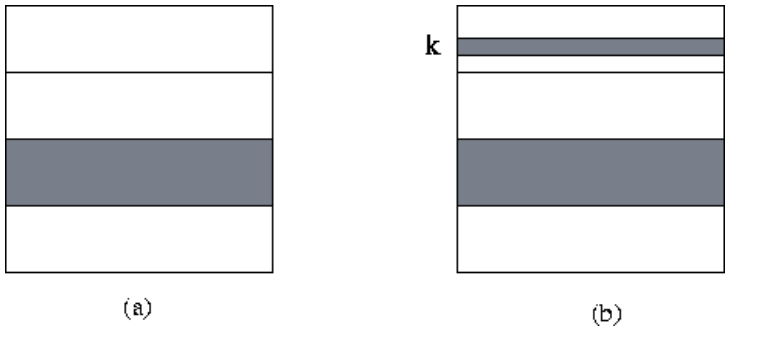
\includegraphics[width=\textwidth]{floyd-openmp}
    \caption{Ukázka dat přidělených jednomu vláknu při paralelizaci jednoho cyklu \cite{w:fw:omp}.}
    \label{f:fw:omp}
\end{figure}


\subsubsection{Druhá varianta}
Druhou variantou, jak problém paralelizovat je použít původní variantu a~přidat paralelizaci zároveň ve vnitřním cyklu, který prochází jednotlivé sloupce matice. V~takovém případě by jednomu vláknu byl přidělen jeden nebo více necelých řádků ohraničených sloupci. Tato varianta se jeví vhodnější pouze při velkém počtu dostupných vláken, proto není v~naší implementaci použita.


\subsection{Měření}
Na obou algoritmech bylo provedeno měření, které si klade za cíl analyzovat čas, zrychlení a~efektivitu použitého paralelního algoritmu. Měření bylo prováděno na hustých grafech, kde při generování grafů byla použita pravděpodobnost 0.5, že mezi dvěmi uzly existuje hrana.

\subsubsection{Testovací data}
Byly vygenerovány 2 testovací sady dat. Obě sady obsahují 25 grafů, kde pro každé $n$ (počet uzlů) z $1000$, $2000$, $3000$, $4000$ a $5000$ 
je vygenerováno 5 náhodných grafů. Jedna sada obsahuje \emph{husté} grafy s~pravděpodobností hrany $50 \%$, druhá obsahuje \emph{řídké} grafy
s~pravděpodobností hrany $1 \%$.
Měření probíhalo na serveru \url{star2.fit.cvut.cz} na stroji \textit{gpu-02} pro počet vláken $p$ $1$, $2$, $4$, $6$, $8$, $12$ a $24$.

Jako čas výpočtu pro dané $n$ se vypočítal průměr z časů přes všech 5 grafů s odpovídajícím počtem uzlů.

\subsubsection{Výsledky}
Grafy \ref{f:mer:cas}, \ref{f:mer:zry} a~\ref{f:mer:efe} ukazují výsledky měření z~pohledu času, zrychlení a~efektivity.

% Cas
\begin{figure}
    \centering
    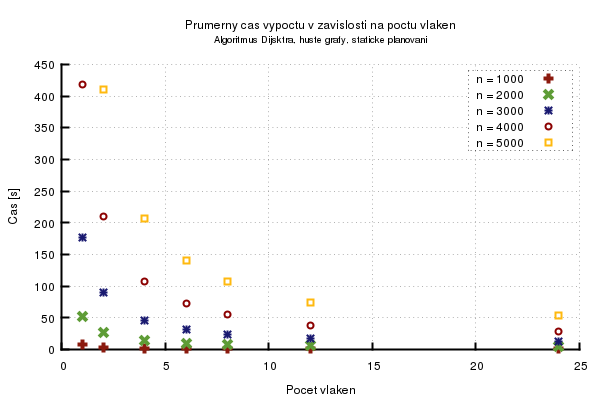
\includegraphics[width=0.45\textwidth]{../grafy/02_openMP/02-01-Dijsktra_cas}
    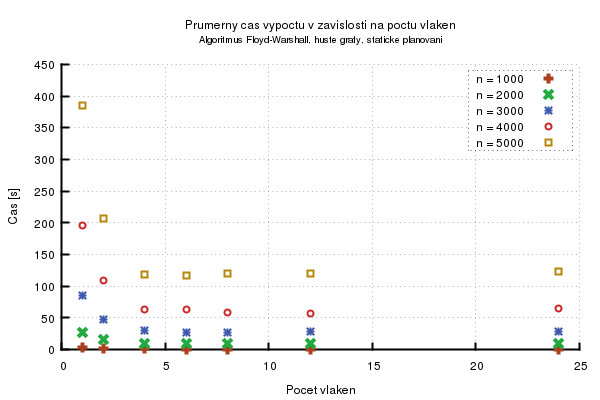
\includegraphics[width=0.45\textwidth]{../grafy/02_openMP/02-01-Floyd_cas}
    \caption{Závislost průměrného času výpočtu v~závislosti na počtu vláken za použití statického plánování.}
    \label{f:mer:cas}
\end{figure}

% Zrychleni
\begin{figure}
    \centering
    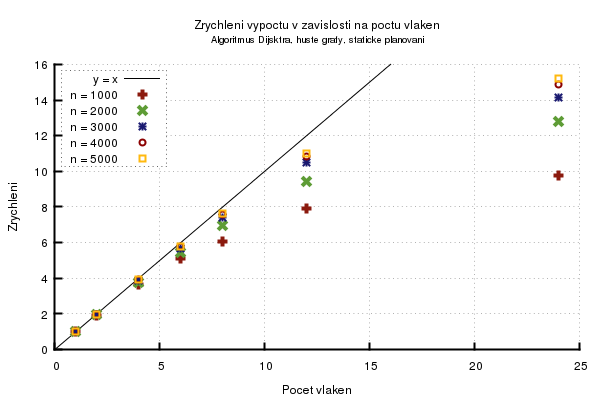
\includegraphics[width=0.45\textwidth]{../grafy/02_openMP/02-02-Dijsktra_zrychleni}
    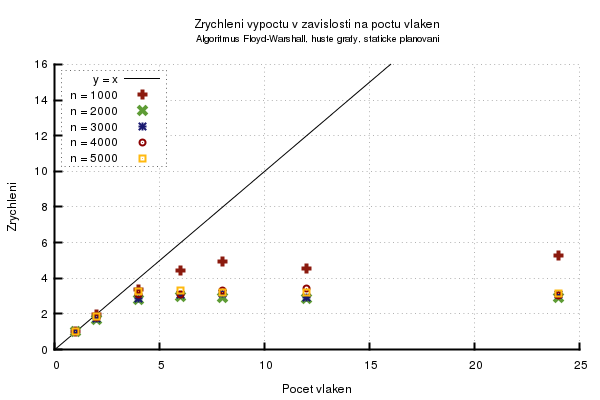
\includegraphics[width=0.45\textwidth]{../grafy/02_openMP/02-02-Floyd_zrychleni}
    \caption{Závislost zrychlení paralelního algoritmu oproti sekvenčnímu v~závislosti na počtu vláken za použití statického plánování.}
    \label{f:mer:zry}
\end{figure}

% Efektivita
\begin{figure}
    \centering
    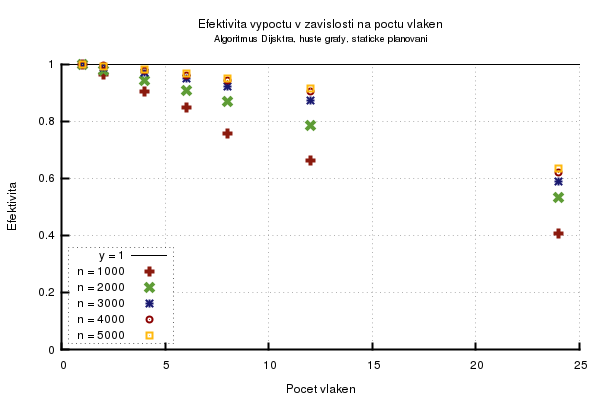
\includegraphics[width=0.45\textwidth]{../grafy/02_openMP/02-03-Dijsktra_efektivita}
    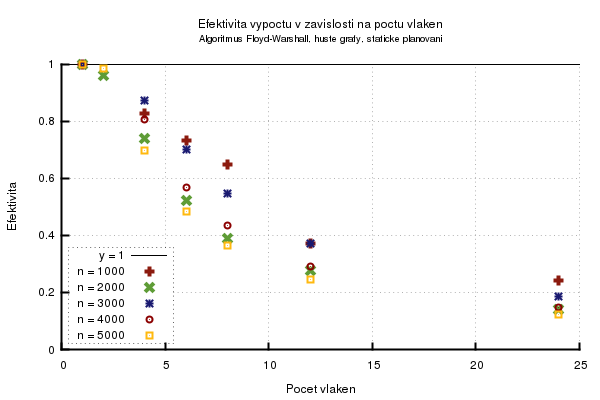
\includegraphics[width=0.45\textwidth]{../grafy/02_openMP/02-03-Floyd_efektivita}
    \caption{Závislost efektivity algoritmu v~závislosti na počtu vláken za použití statického plánování.}
    \label{f:mer:efe}
\end{figure}

\paragraph{Poměr rychlosti algoritmů v závislosti na hustotě grafu}
Graf \ref{f:mer:pomerhustota} porovnává výpočetní časy při použití statického plánování v závislosti na hustotě grafu. Z grafů vyplývá, že oba algoritmy jsou téměř nezávislé na hustotě grafu.

\paragraph{Poměr rychlosti algoritmů v závislosti na plánování}
Graf \ref{f:mer:pomerplanovani} zobrazuje poměr výpočetních časů v závislosti na použitém plánování. V porovnání byla použita plánování statické a dynamické. Z grafů je patrné, že plánování ovlivní čas výpočtu pouze nevýznamně a není tedy podstatné, jaké plánování je v algoritmu použito.
\paragraph{Statické plánování}
Při statickém plánování se iterace cyklu rovnoměrně rozdělí po blocích mezi všechna vlákna před začátkem provádění cyklu \cite{w:omp}.
\paragraph{Dynamické plánování}
Dynamickým plánováním se rozumí rozdělení jednotlivých iterací vláknům po jedné iteraci. Vždy když vlákno dokončí iteraci, je mu přidělena další iterace \cite{w:omp}.

% Pomer rychlost vypoctu v zavislosti na hustote grafu
\begin{figure}
    \centering
    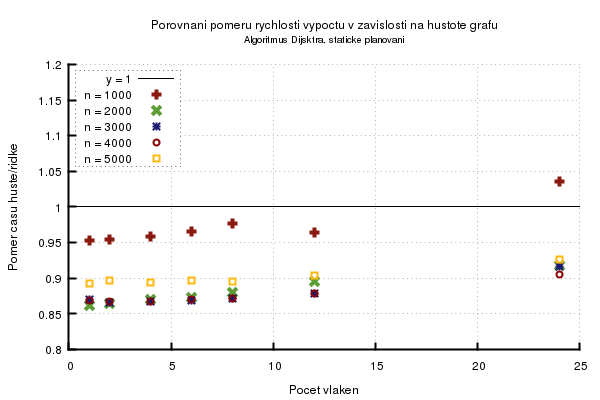
\includegraphics[width=0.45\textwidth]{../grafy/02_openMP/02-04-Dijsktra_hustota}
    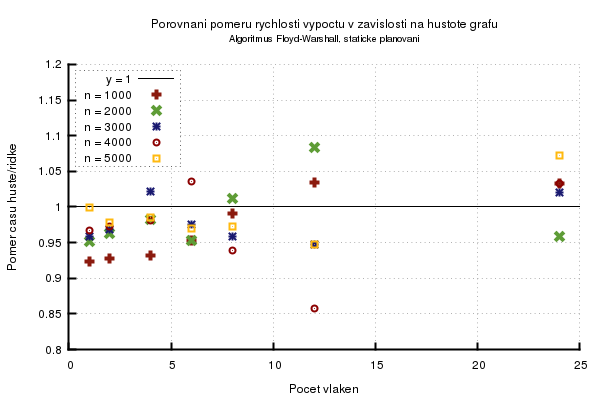
\includegraphics[width=0.45\textwidth]{../grafy/02_openMP/02-04-Floyd_hustota}
    \caption{Porovnání poměru rychlostí výpočtu v závislosti na hustotě grafu při použití statického plánování.}
    \label{f:mer:pomerhustota}
\end{figure}

% Pomer rychlost vypoctu v zavislosti na hustote grafu
\begin{figure}
    \centering
    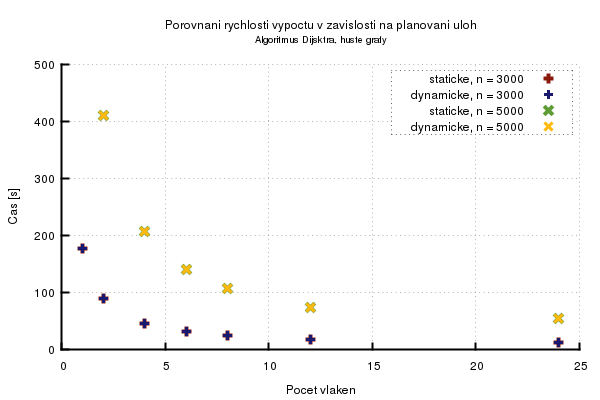
\includegraphics[width=0.45\textwidth]{../grafy/02_openMP/02-05-Dijsktra_schedule}
    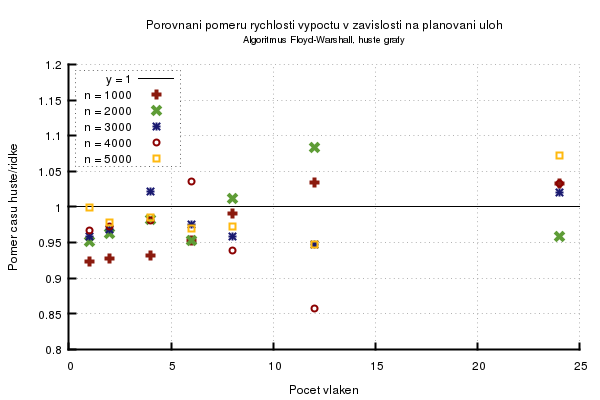
\includegraphics[width=0.45\textwidth]{../grafy/02_openMP/02-05-Floyd_schedule}
    \caption{Porovnání poměru rychlostí výpočtu v závislosti na použitém plánování.}
    \label{f:mer:pomerplanovani}
\end{figure}

\subsubsection{Analýza}
\paragraph{Dijsktra}
Z~grafů \ref{f:mer:cas} je vidět klesající dobu výpočtu v závislosti na počtu vláken.
Zrychlení, které je zobrazeno v~grafu \ref{f:mer:zry} na počátku stoupá téměř lineárně a~teprve pro větší počet vláken 
se zmírňuje. Toto nelineární zrychlení může způsobit například přístup do paměti, protože se vzrůstajícím počtem vláken klesá 
relativní velikost cache pro každé z vláken.
Z~výše uvedeného vyplývá efektivita, která je zobrazena v~grafu \ref{f:mer:efe}.

\paragraph{Floyd-Warshallův algoritmus}
U~Floyd-Warshallova algoritmu se výpočetní čas pro počty vláken větší než 3 téměř nezkracuje. 
Zrychlení je tedy patrné pouze při použití 2 případně 4 vláknech. Z~výše uvedené plyne, že efektivita paralelního algoritmu velmi rychle klesá.

\subsubsection{Zhodnocení}
Efektivita Dijkstrova algoritmu s~přidáváním vláken pomalu klesá a~například pro 24 vláken dosahuje hodnoty 0.5. Naproti tomu u~Floyd-Warshallova algoritmu klesá efektivita mnohem rychleji a~na hodnotě 0.5 se nachází už pro 6 vláken. 

Výrazně lépe ve prospěch Dijkstrova paralelního algoritmu vycházejí i~ostatní ukazatele -- zrychlení a~čas výpočtu.

Výsledky Floyd-Warshallova algoritmu mohou být způsobeny opakovaným vytvářením a~rušením vláken. V~každém vnějším cyklu se vytvoří daný počet vláken, zpracuje jeden uzel a~všechna tato vytvořená vlákna se opět ukončí. Tedy za běhu algoritmu se vytváří a~ruší \textit{pocet\_uzlu $\times$ vlaken}, kde parametr \textit{vlaken} je počet najednou vytvářených paralelních vláken.



%-------------------------------
%---		CUDA			 ---
%-------------------------------
%\section{Paralelní algoritmus pomocí technologie CUDA}
%\subsection{Dijkstrův algoritmus}
%\subsubsection{Úprava algoritmu}
%\subsubsection{Optimalizace}
%
%\subsection{Floyd-Warshallův algoritmus}
%\subsubsection{Úprava algoritmu}
%\subsubsection{Optimalizace}
%
%\subsection{Měření}
%\subsubsection{Analýza}
%\subsubsection{Zhodnocení}
%
%
%\section{Závěr}




\clearpage
\bibliographystyle{czechiso} % nutny soubor czechiso.bst
\bibliography{citace}

\end{document}
